\chapter{Alguns Exemplos de Comandos \LaTeX{}}
\label{chap:exemplos}

\section{Bibliografia e Referências}

A documentação do pacote biblatex\index{biblatex} é bastante extensa e explica
os diversos tipos de documento suportados, bem como o significado
de cada campo. Na prática, às vezes é preciso fazer escolhas sobre
o que incluir na descrição de um item bibliográfico e muitas vezes
é mais fácil aprender copiando exemplos já existentes, como estes (consulte o
arquivo \texttt{bibliografia.bib} para ver como foi criado o banco de dados e a
bibliografia na página \pageref{bibliografia} para ver o resultado impresso):

\begin{multicols}{2}
  \begin{itemize}
    \item @Book: \cite{JW82}.

    \item @Article: \cite{MenaChalco08}.

    \item @InProceedings: \cite{alves03:simi}.

    \item @Conference (sinônimo de @InProceedings): \cite{bronevetsky02}.

    \item @InCollection: \cite{bobaoglu93:concepts}.

    \item @PhdThesis: \cite{garcia01:PhD}.

    \item @MastersThesis: \cite{schmidt03:MSc}.

    \item @Techreport: \cite{alvisi99:analysisCIC}.

    \item @Manual: \cite{CORBA:spec}.

    \item @Misc: \cite{gridftp}.

    \item @Online (para referência a artigo \emph{online}): \cite{fowler04:designDead}.

    \item @Online (para referência a página web): \cite{FSF:GNU-GPL}.
  \end{itemize}
\end{multicols}

\section{Modo Matemático}\index{Modo Matemático}

O modo matemático do \LaTeX{} tem sintaxe própria, mas ela não é complicada e
há bastante documentação \emph{online} a respeito. Por exemplo, ``massa e
energia são grandezas relacionadas pela Equação $E=mc^2$, definida inicialmente
por Einstein'', ou ainda ``equações de segundo grau (Equação \ref{eq:2grau})
são estudadas no ensino médio. As raízes de uma equação de segundo grau podem
ser encontradas por~\eqref{eq:bhaskara} --- a fórmula de Bháskara.
O valor do discriminante $\Delta$ (Equação \ref{eq:delta}) determina se a
equação tem zero, uma ou duas raízes reais''. Observe que, quando um
parágrafo termina com um símbolo, pode ser boa ideia usar um espaço
não-separável (com ``\textsf{\textasciitilde}'') para evitar que ele
fique sozinho na última linha (por exemplo, ``\textsf{O discriminante é
denotado por\textasciitilde{}\$\textbackslash{}Delta\$}'').\label{orphanchar}

\begin{equation}
  \label{eq:2grau}
  ax^2+bx+c=y \quad \forall x \in \mathbb{R}
\end{equation}

\begin{gather}
  \label{eq:bhaskara}
    y=0 \Leftrightarrow x=\frac{-b \pm \sqrt{\Delta}}{2a}
    \Leftrightarrow x \text{ é raiz da equação}\\
  \label{eq:delta}
    \Delta\enspace(\mathit{delta}) = b^2-4ac
\end{gather}

\section{\emph{Floats} (Tabelas e Figuras)}\index{Floats}

Evidentemente, \LaTeX{} permite inserir figuras no texto; além disso, ele
também permite girá-las e criar subfiguras (com sublegendas\index{Legendas}),
como no exemplo da Figura~\ref{fig:subfigures}\index{Subfiguras}, que inclui
as subfiguras \ref{fig:subfigures:a} e \ref{fig:subfigures:b}. Uma
``figura'', na verdade, pode ser qualquer tipo de conteúdo ilustrativo
(como no caso da Figura~\ref{fig:gantt}, que é um cronograma) mas, com a
\textit{package} \textsf{float}, também é possível definir ambientes
específicos para cada tipo de conteúdo adicional (cada um com numeração
independente), como é o caso do Programa~\ref{prog:java}\index{Floats}. Há
mais informações e dicas sobre recursos específicos para inclusão de
código-fonte e pseudocódigo no Apêndice \ref{ap:pseudocode}\footnote{
Observe que o nome do Apêndice (``\ref{ap:pseudocode}'') foi impresso em
uma linha separada, o que não é muito bom visualmente. Para evitar que isso
aconteça (não só no final do parágrafo, mas em qualquer quebra de linha),
faça o que já foi discutido na Seção~\ref{orphanchar} sobre símbolos
matemáticos: utilize um espaço não-separável para fazer referências a
figuras, tabelas, seções etc.: ``\textsf{\dots no
Apêndice\textasciitilde\textbackslash{}ref\{ap:pseudocode\}}''.}.

% As packages relevantes para lidar com figuras são graphicx,
% float, caption, rotating e subcaption. Observe que "subfigure"
% e "subtable" são definidos na package subcaption, *não* na
% package subfigure! A package subfigure é obsoleta.

%%%%%%%%% Figuras lado-a-lado %%%%%%%%%
\begin{figure}
  \centering

  \begin{subfigure}{0.4\textwidth}
    \centering
    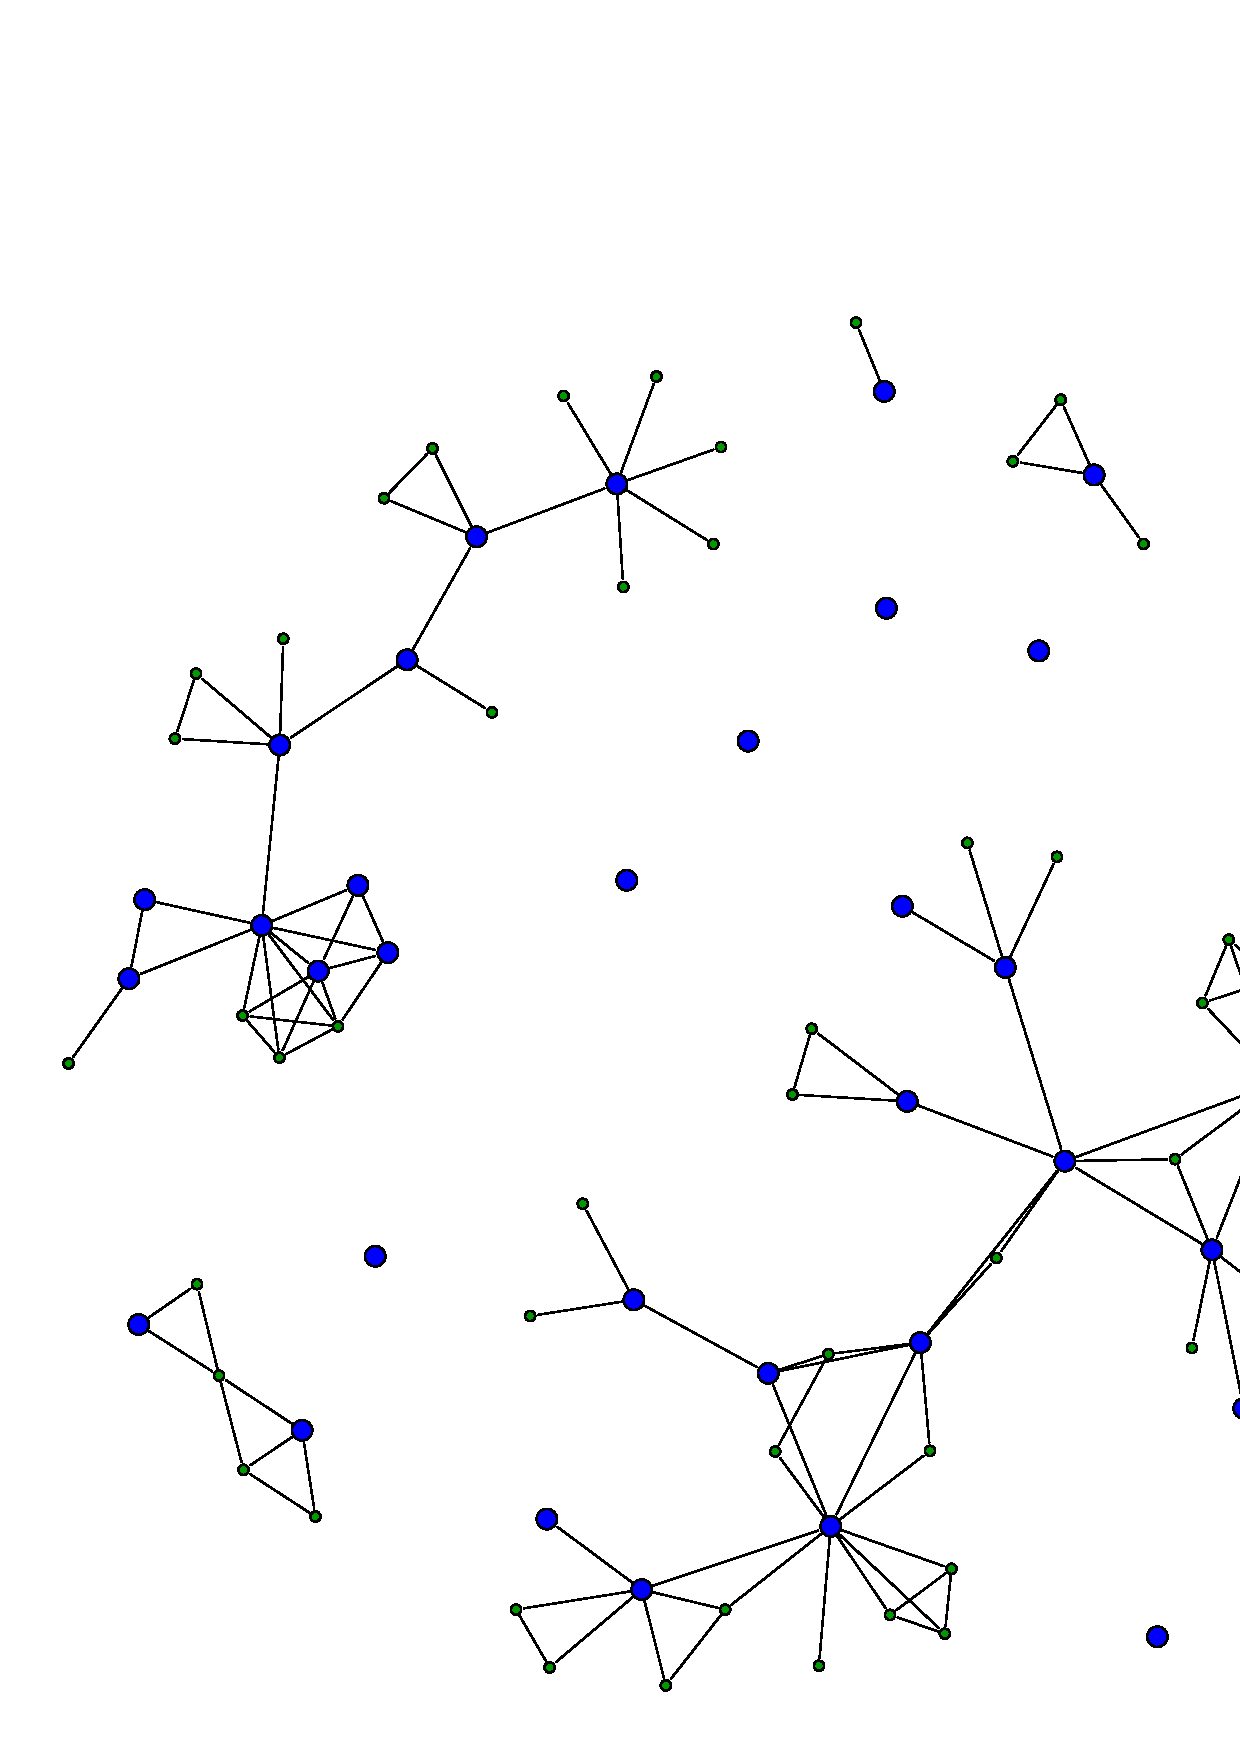
\includegraphics[width=.7\textwidth]{graph}
    \caption{Uma figura simples.\label{fig:subfigures:a}}
  \end{subfigure}
  % ATENÇÃO: Se você deixar uma linha em branco entre as subfiguras,
  % LaTeX vai considerar que cada uma delas pertence a um "parágrafo"
  % diferente e, portanto, vai colocá-las em linhas separadas ao invés
  % de lado a lado.
  \begin{subfigure}{0.4\textwidth}
    \centering
    \begin{turn}{90}
      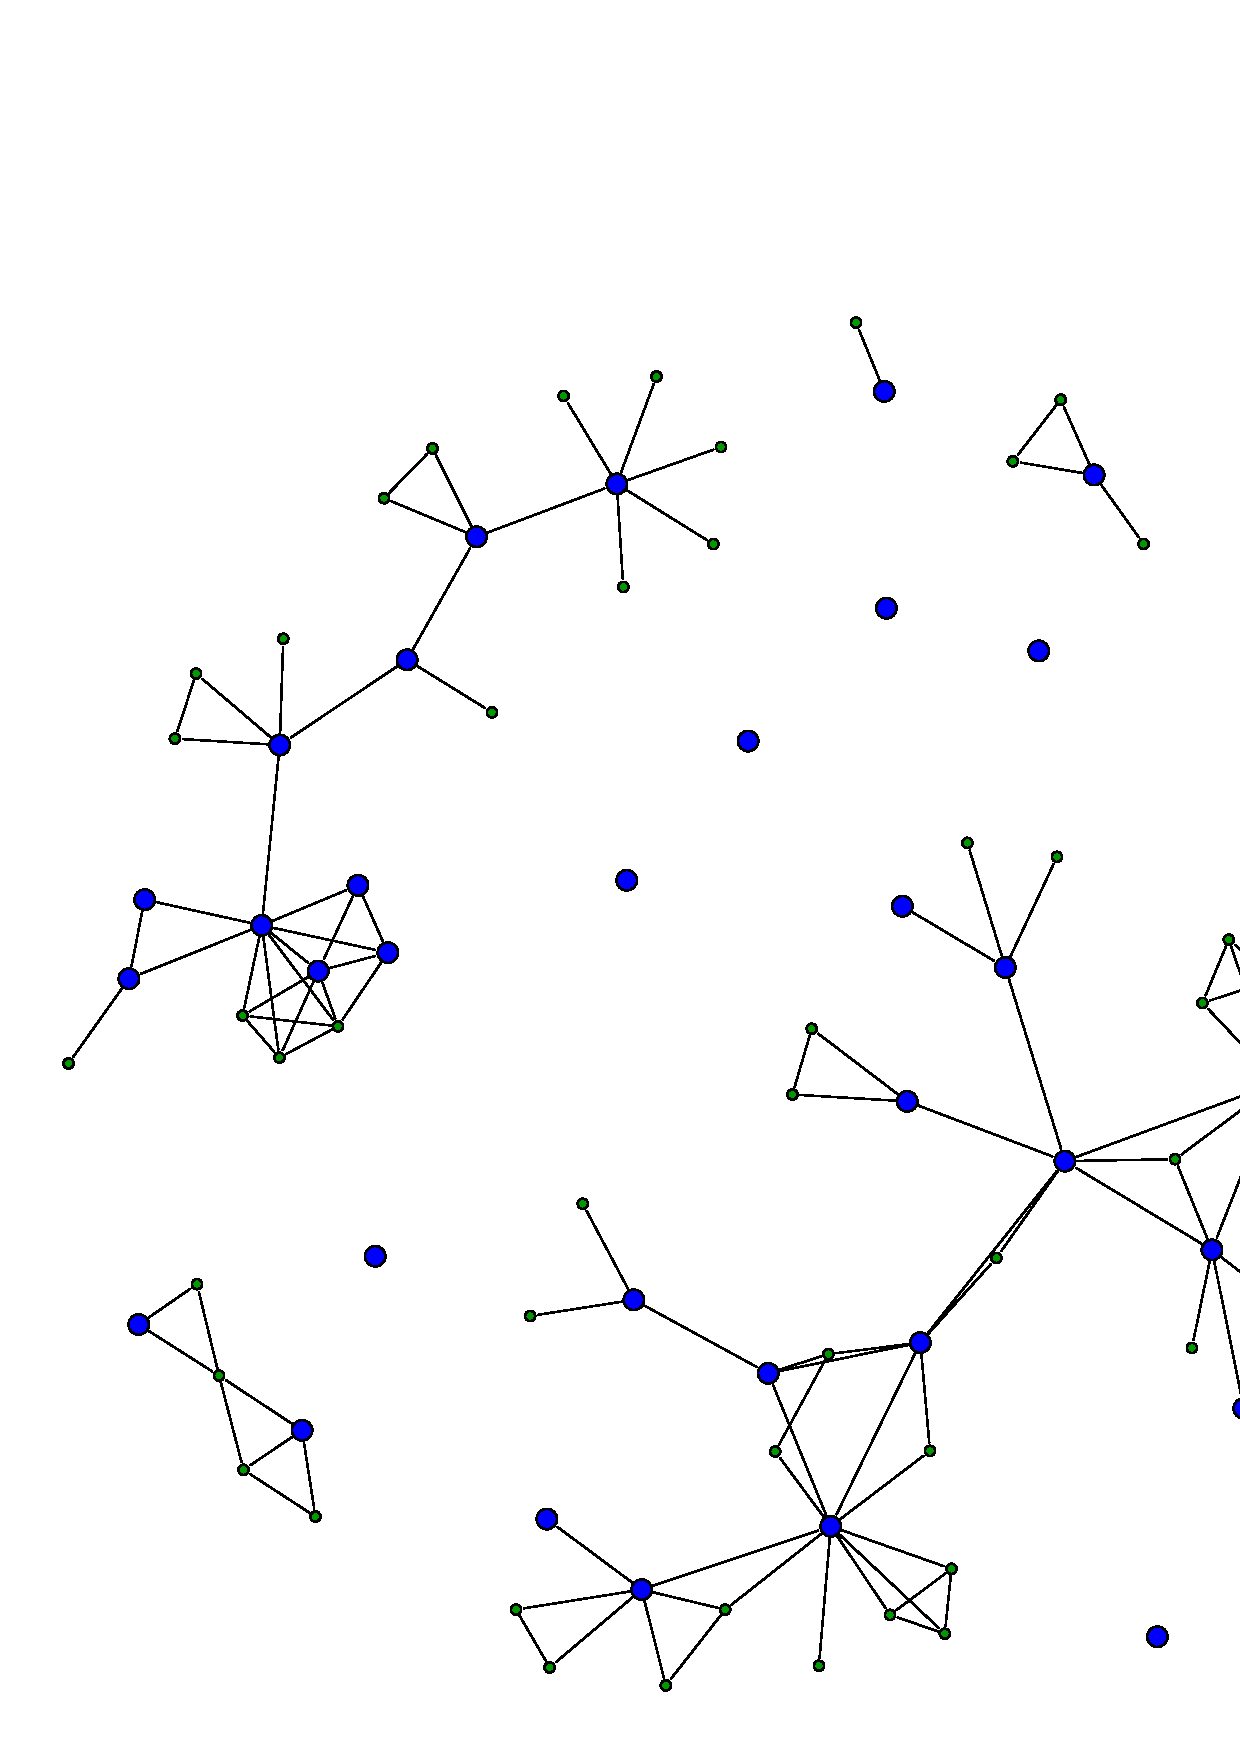
\includegraphics[width=.7\textwidth]{graph}
    \end{turn}
    \caption{O mesmo exemplo, girado.\label{fig:subfigures:b}}
  \end{subfigure}

  \caption{Exemplo de subfiguras.\label{fig:subfigures}}
\end{figure}

%%%%%%%% Código fonte %%%%%%%%

% Foi utilizado o pacote listings para formatar o código fonte.
% Veja os parâmetros de configuração no arquivo source-code.tex.
\begin{program}
  \index{Java}
  \centering

\begin{lstlisting}[language=Java, style=wider]
  for (i = 0; i < 20; i++)
  {
      // Comentário
      System.out.println("Mensagem...");
  }
\end{lstlisting}

  \caption{Exemplo de laço em Java.\label{prog:java}}
\end{program}

%%%%%%% Cronograma %%%%%%%

\begin{figure}
  \centering

  \begin{ganttchart}{2017-11}{2018-5}
    \gantttitlecalendar{year,month=shortname} \ganttnewline

    \ganttgroup[progress=45]{Experimento}{2017-11}{2018-2} \ganttnewline
    \ganttbar[progress=100]{
      Preparação\ganttalignnewline
      (compra de insumos)
      }{2017-11}{2017-12} \ganttnewline
    \ganttbar[progress=30]{Execução}{2017-12}{2018-1} \ganttnewline
    \ganttbar[progress=0]{Análise}{2017-12}{2018-2} \ganttnewline

    \ganttgroup[progress=0]{Artigo}{2018-1}{2018-4} \ganttnewline
    \ganttbar[progress=0]{Escrita}{2018-1}{2018-3} \ganttnewline
    \ganttbar[progress=0]{Revisão}{2018-3}{2018-4} \ganttnewline

    \ganttmilestone{Submissão}{2018-4}
  \end{ganttchart}

  \caption{Exemplo de cronograma.\label{fig:gantt}}
\end{figure}

%%%%%

Talvez você precise organizar a apresentação da informação na forma de
tabelas\index{Floats}; um exemplo simples é a Tabela~\ref{tab:amino_acidos}.

%%%%%%%% Tabelas lado-a-lado %%%%%%%%

\begin{table}
\centering

  \hspace*{\fill}
  \begin{subtable}[b]{0.42\textwidth}
    \centering
    \begin{tabular}{ccl}
      \toprule
      Código      & Abreviatura  & \makecell{Nome\\completo} \\
      \midrule
      \texttt{A}  & Ala          & Alanina \\
      \texttt{C}  & Cys          & Cisteína \\
      ...         & ...          & ... \\
      \texttt{W}  & Trp          & Triptofano \\
      \texttt{Y}  & Tyr          & Tirosina \\
      \bottomrule
    \end{tabular}
    \caption{Uma tabela simples.}
  \end{subtable}
  % Como mencionado mais acima, não deixe linhas em branco aqui
  \hspace*{\fill}\hspace*{\fill}\hspace*{\fill}
  \begin{subtable}[b]{0.37\textwidth}
    \centering
    \begin{tabular}{ccl}
      \rothead{Código} & \rothead{Abreviatura} & \rothead{Nome\\completo} \\
      \midrule
      \texttt{A}       & Ala                   & Alanina \\
      \texttt{C}       & Cys                   & Cisteína \\
      ...              & ...                   & ... \\
      \texttt{W}       & Trp                   & Triptofano \\
      \texttt{Y}       & Tyr                   & Tirosina \\
      \bottomrule
    \end{tabular}
    \caption{Com cabeçalhos girados.}
  \end{subtable}
  \hspace*{\fill}

  \caption{Códigos, abreviaturas e nomes dos aminoácidos.\label{tab:amino_acidos}}
\end{table}

Se a tabela tem muitas linhas e, portanto, não cabe em uma única página, é
possível fazê-la continuar ao longo de várias páginas com a \textit{package}
\textsf{longtable}, como é o caso da Tabela~\ref{tab:numeros}. Nesse caso,
a tabela não é um \textit{float} e, portanto, ela aparece de acordo com a
sequência normal do texto. Se, além de muito longa, a tabela for também
muito larga, você pode usar o comando \textsf{landscape} (da
\textit{package} \textsf{pdflscape}) em conjunto com \textsf{longtable}
para imprimi-la em modo paisagem ao longo de várias páginas. A
Tabela~\ref{tab:numeros} tem essa configuração comentada; experimente
des-comentar as linhas correspondentes\footnote{Observe que, nesse caso,
vai sempre haver uma quebra de página no texto para fazer a tabela
começar em uma página em modo paisagem.}.

%%%%%%%% Tabela longa em várias páginas %%%%%%%%

%%%% É possível fazer esta mesma tabela em modo paisagem des-comentando
%%%% esta linha e a correspondente no final da tabela
%\begin{landscape}
\begin{center}
\begin{longtable}{|c|c|c|c|c|c|c|c|c|c|c|c|c|}
 % O label não deve ficar em um cabeçalho que se repete!
\caption{Exemplo de tabela com valores numéricos.\label{tab:numeros}}\\
\hline
\emph{Lim.} &
\multicolumn{3}{c|}{MGWT} &
\multicolumn{3}{c|}{AMI} &
\multicolumn{3}{c|}{\emph{Spectrum} de Fourier} &
\multicolumn{3}{c|}{Caract. espectrais} \\
\cline{2-4} \cline{5-7} \cline{8-10} \cline{11-13} &
\emph{Sn} & \emph{Sp} & \emph{AC} &
\emph{Sn} & \emph{Sp} & \emph{AC} &
\emph{Sn} & \emph{Sp} & \emph{AC} &
\emph{Sn} & \emph{Sp} & \emph{AC} \\
\hline \hline
\endfirsthead
% Final do cabeçalho que aparece na primeira página; neste caso,
% igual ao das páginas seguintes, definido logo abaixo, exceto
% pelo comando caption; essa diferença impede que a lista de
% tabelas inclua uma referência para cada página da tabela

\caption[]{Exemplo de tabela com valores numéricos (cont.).}\\
\hline
\emph{Lim.} &
\multicolumn{3}{c|}{MGWT} &
\multicolumn{3}{c|}{AMI} &
\multicolumn{3}{c|}{\emph{Spectrum} de Fourier} &
\multicolumn{3}{c|}{Caract. espectrais} \\
\cline{2-4} \cline{5-7} \cline{8-10} \cline{11-13} &
\emph{Sn} & \emph{Sp} & \emph{AC} &
\emph{Sn} & \emph{Sp} & \emph{AC} &
\emph{Sn} & \emph{Sp} & \emph{AC} &
\emph{Sn} & \emph{Sp} & \emph{AC} \\
\hline \hline
\endhead % Final do cabeçalho que aparece em todas as páginas

\hline
\multicolumn{13}{|r|}{\textit{continua}\enspace$\longrightarrow$}\\
\hline
\endfoot % Final do rodapé que aparece em todas as páginas exceto a última

\hline
\endlastfoot % Final do rodapé da última página (neste caso, apenas uma linha)
 1 & 1.00 & 0.16 & 0.08 & 1.00 & 0.16 & 0.08 & 1.00 & 0.16 & 0.08 & 1.00 & 0.16 & 0.08 \\
 2 & 1.00 & 0.16 & 0.09 & 1.00 & 0.16 & 0.09 & 1.00 & 0.16 & 0.09 & 1.00 & 0.16 & 0.09 \\
 3 & 1.00 & 0.16 & 0.10 & 1.00 & 0.16 & 0.10 & 1.00 & 0.16 & 0.10 & 1.00 & 0.16 & 0.10 \\
 4 & 1.00 & 0.16 & 0.10 & 1.00 & 0.16 & 0.10 & 1.00 & 0.16 & 0.10 & 1.00 & 0.16 & 0.10 \\
 5 & 1.00 & 0.16 & 0.11 & 1.00 & 0.16 & 0.11 & 1.00 & 0.16 & 0.11 & 1.00 & 0.16 & 0.11 \\
 6 & 1.00 & 0.16 & 0.12 & 1.00 & 0.16 & 0.12 & 1.00 & 0.16 & 0.12 & 1.00 & 0.16 & 0.12 \\
 7 & 1.00 & 0.17 & 0.12 & 1.00 & 0.17 & 0.12 & 1.00 & 0.17 & 0.12 & 1.00 & 0.17 & 0.13 \\
 8 & 1.00 & 0.17 & 0.13 & 1.00 & 0.17 & 0.13 & 1.00 & 0.17 & 0.13 & 1.00 & 0.17 & 0.13 \\
 9 & 1.00 & 0.17 & 0.14 & 1.00 & 0.17 & 0.14 & 1.00 & 0.17 & 0.14 & 1.00 & 0.17 & 0.14 \\
10 & 1.00 & 0.17 & 0.15 & 1.00 & 0.17 & 0.15 & 1.00 & 0.17 & 0.15 & 1.00 & 0.17 & 0.15 \\
11 & 1.00 & 0.17 & 0.15 & 1.00 & 0.17 & 0.15 & 1.00 & 0.17 & 0.15 & 1.00 & 0.17 & 0.15 \\
12 & 1.00 & 0.18 & 0.16 & 1.00 & 0.18 & 0.16 & 1.00 & 0.18 & 0.16 & 1.00 & 0.18 & 0.16 \\
13 & 1.00 & 0.18 & 0.17 & 1.00 & 0.18 & 0.17 & 1.00 & 0.18 & 0.17 & 1.00 & 0.18 & 0.17 \\
14 & 1.00 & 0.18 & 0.17 & 1.00 & 0.18 & 0.17 & 1.00 & 0.18 & 0.17 & 1.00 & 0.18 & 0.17 \\
15 & 1.00 & 0.18 & 0.18 & 1.00 & 0.18 & 0.18 & 1.00 & 0.18 & 0.18 & 1.00 & 0.18 & 0.18 \\
16 & 1.00 & 0.18 & 0.19 & 1.00 & 0.18 & 0.19 & 1.00 & 0.18 & 0.19 & 1.00 & 0.18 & 0.19 \\
17 & 1.00 & 0.19 & 0.19 & 1.00 & 0.19 & 0.19 & 1.00 & 0.19 & 0.19 & 1.00 & 0.19 & 0.19 \\
18 & 1.00 & 0.19 & 0.20 & 1.00 & 0.19 & 0.20 & 1.00 & 0.19 & 0.20 & 1.00 & 0.19 & 0.20 \\
19 & 1.00 & 0.19 & 0.21 & 1.00 & 0.19 & 0.21 & 1.00 & 0.19 & 0.21 & 1.00 & 0.19 & 0.21 \\
20 & 1.00 & 0.19 & 0.22 & 1.00 & 0.19 & 0.22 & 1.00 & 0.19 & 0.22 & 1.00 & 0.19 & 0.22 \\
21 & 1.00 & 0.19 & 0.22 & 1.00 & 0.19 & 0.22 & 1.00 & 0.19 & 0.22 & 1.00 & 0.19 & 0.22 \\
22 & 1.00 & 0.19 & 0.22 & 1.00 & 0.19 & 0.22 & 1.00 & 0.19 & 0.22 & 1.00 & 0.19 & 0.22 \\
23 & 1.00 & 0.19 & 0.22 & 1.00 & 0.19 & 0.22 & 1.00 & 0.19 & 0.22 & 1.00 & 0.19 & 0.22 \\
24 & 1.00 & 0.19 & 0.22 & 1.00 & 0.19 & 0.22 & 1.00 & 0.19 & 0.22 & 1.00 & 0.19 & 0.22 \\
25 & 1.00 & 0.19 & 0.22 & 1.00 & 0.19 & 0.22 & 1.00 & 0.19 & 0.22 & 1.00 & 0.19 & 0.22 \\
26 & 1.00 & 0.19 & 0.22 & 1.00 & 0.19 & 0.22 & 1.00 & 0.19 & 0.22 & 1.00 & 0.19 & 0.22 \\
27 & 1.00 & 0.19 & 0.22 & 1.00 & 0.19 & 0.22 & 1.00 & 0.19 & 0.22 & 1.00 & 0.19 & 0.22 \\
28 & 1.00 & 0.19 & 0.22 & 1.00 & 0.19 & 0.22 & 1.00 & 0.19 & 0.22 & 1.00 & 0.19 & 0.22 \\
29 & 1.00 & 0.19 & 0.22 & 1.00 & 0.19 & 0.22 & 1.00 & 0.19 & 0.22 & 1.00 & 0.19 & 0.22 \\
30 & 1.00 & 0.19 & 0.22 & 1.00 & 0.19 & 0.22 & 1.00 & 0.19 & 0.22 & 1.00 & 0.19 & 0.22 \\
31 & 1.00 & 0.19 & 0.22 & 1.00 & 0.19 & 0.22 & 1.00 & 0.19 & 0.22 & 1.00 & 0.19 & 0.22 \\
% Como nesta página há uma nota de rodapé, a linha separadora da nota
% e a linha final da tabela ficam muito próximas; vamos forçar uma
% quebra de página uma linha antes para resolver isso.
\pagebreak
32 & 1.00 & 0.19 & 0.22 & 1.00 & 0.19 & 0.22 & 1.00 & 0.19 & 0.22 & 1.00 & 0.19 & 0.22 \\
33 & 1.00 & 0.19 & 0.22 & 1.00 & 0.19 & 0.22 & 1.00 & 0.19 & 0.22 & 1.00 & 0.19 & 0.22 \\
34 & 1.00 & 0.19 & 0.22 & 1.00 & 0.19 & 0.22 & 1.00 & 0.19 & 0.22 & 1.00 & 0.19 & 0.22 \\
35 & 1.00 & 0.19 & 0.22 & 1.00 & 0.19 & 0.22 & 1.00 & 0.19 & 0.22 & 1.00 & 0.19 & 0.22 \\
36 & 1.00 & 0.19 & 0.22 & 1.00 & 0.19 & 0.22 & 1.00 & 0.19 & 0.22 & 1.00 & 0.19 & 0.22 \\
37 & 1.00 & 0.19 & 0.22 & 1.00 & 0.19 & 0.22 & 1.00 & 0.19 & 0.22 & 1.00 & 0.19 & 0.22 \\
38 & 1.00 & 0.19 & 0.22 & 1.00 & 0.19 & 0.22 & 1.00 & 0.19 & 0.22 & 1.00 & 0.19 & 0.22 \\
39 & 1.00 & 0.19 & 0.22 & 1.00 & 0.19 & 0.22 & 1.00 & 0.19 & 0.22 & 1.00 & 0.19 & 0.22 \\
40 & 1.00 & 0.19 & 0.22 & 1.00 & 0.19 & 0.22 & 1.00 & 0.19 & 0.22 & 1.00 & 0.19 & 0.22 \\
41 & 1.00 & 0.19 & 0.22 & 1.00 & 0.19 & 0.22 & 1.00 & 0.19 & 0.22 & 1.00 & 0.19 & 0.22 \\
42 & 1.00 & 0.19 & 0.22 & 1.00 & 0.19 & 0.22 & 1.00 & 0.19 & 0.22 & 1.00 & 0.19 & 0.22 \\
43 & 1.00 & 0.19 & 0.22 & 1.00 & 0.19 & 0.22 & 1.00 & 0.19 & 0.22 & 1.00 & 0.19 & 0.22 \\
44 & 1.00 & 0.19 & 0.22 & 1.00 & 0.19 & 0.22 & 1.00 & 0.19 & 0.22 & 1.00 & 0.19 & 0.22 \\
45 & 1.00 & 0.19 & 0.22 & 1.00 & 0.19 & 0.22 & 1.00 & 0.19 & 0.22 & 1.00 & 0.19 & 0.22 \\
46 & 1.00 & 0.19 & 0.22 & 1.00 & 0.19 & 0.22 & 1.00 & 0.19 & 0.22 & 1.00 & 0.19 & 0.22 \\
47 & 1.00 & 0.19 & 0.22 & 1.00 & 0.19 & 0.22 & 1.00 & 0.19 & 0.22 & 1.00 & 0.19 & 0.22 \\
48 & 1.00 & 0.19 & 0.22 & 1.00 & 0.19 & 0.22 & 1.00 & 0.19 & 0.22 & 1.00 & 0.19 & 0.22 \\
49 & 1.00 & 0.19 & 0.22 & 1.00 & 0.19 & 0.22 & 1.00 & 0.19 & 0.22 & 1.00 & 0.19 & 0.22 \\
50 & 1.00 & 0.19 & 0.22 & 1.00 & 0.19 & 0.22 & 1.00 & 0.19 & 0.22 & 1.00 & 0.19 & 0.22 \\
51 & 1.00 & 0.19 & 0.22 & 1.00 & 0.19 & 0.22 & 1.00 & 0.19 & 0.22 & 1.00 & 0.19 & 0.22 \\
52 & 1.00 & 0.19 & 0.22 & 1.00 & 0.19 & 0.22 & 1.00 & 0.19 & 0.22 & 1.00 & 0.19 & 0.22 \\
53 & 1.00 & 0.19 & 0.22 & 1.00 & 0.19 & 0.22 & 1.00 & 0.19 & 0.22 & 1.00 & 0.19 & 0.22 \\
54 & 1.00 & 0.19 & 0.22 & 1.00 & 0.19 & 0.22 & 1.00 & 0.19 & 0.22 & 1.00 & 0.19 & 0.22 \\
55 & 1.00 & 0.19 & 0.22 & 1.00 & 0.19 & 0.22 & 1.00 & 0.19 & 0.22 & 1.00 & 0.19 & 0.22 \\

\end{longtable}
\end{center}
%\end{landscape}

Tabelas mais complexas são um tanto trabalhosas em \LaTeX{}; a
Tabela~\ref{tab:ficha} mostra como construir uma tabela em forma de ficha.
Além de complexa, ela é larga e, portanto, deve ser impressa em modo
paisagem. No entanto, usamos um outro mecanismo para girar a tabela: o
comando \textsf{sidewaystable} (da \textit{package} \textsf{rotating}).
Com esse mecanismo, ela continua sendo um \textit{float} (e, portanto,
não força quebras de página no meio do texto), mas sempre é impressa em
uma página separada.

Resumindo:

\begin{itemize}
  \item Se uma tabela cabe em uma página, defina-a como um \textit{float};
  \item se cabe em uma página mas é muito larga e precisa ser impressa em
        modo paisagem, use \textsf{sidewaystable} (que também é um \textit{float});
  \item se não cabe em uma página por ser muito longa, use \textsf{longtable};
  \item se não cabe em uma página por ser muito longa e precisa ser impressa
        em modo paisagem por ser muito larga, use \textsf{longtable} em
        conjunto com \textsf{landscape}.
\end{itemize}

%%%%%%%% Tabela em forma de ficha %%%%%%%%

% Aumenta o espaçamento entre as linhas da tabela (default: 0pt)
\setlength\extrarowheight{4pt}

% sidewaystable e comandos relacionados são definidos na package rotating
\begin{sidewaystable}
\centering

\begin{tabular}{|M{0.265}|M{0.073}|M{0.084}|M{0.073}|M{0.073}|M{0.08}|M{0.082}|M{0.067}|}
  \hline
    \textbf{Experimento número:} & \multicolumn{2}{c|}{1} & \multicolumn{4}{c|}{\textbf{Data:}} & jan 2017
  \tabularnewline \hline
    \textbf{Título:} & \multicolumn{7}{c|}{Medições iniciais}
  \tabularnewline \hline
    \textbf{Tipo de experimento:} & \multicolumn{7}{c|}{Levantamento quantitativo}
  \tabularnewline \hline \hline
    \textbf{Locais}          & São Paulo & Rio de Janeiro & Porto Alegre & Recife & Manaus & Brasília & Rio Branco
  \tabularnewline \thickhline
    \textbf{Valores obtidos} & 0.2       & 0.3            & 0.2          & 0.7    & 0.5    & 0.1      & 0.4
  \tabularnewline \hline
\end{tabular}

\caption{Exemplo de tabela similar a uma ficha.\label{tab:ficha}}
\end{sidewaystable}

% Redefinindo para o valor default
\setlength\extrarowheight{0pt}
